\subsection{Circuits}\label{sec:circuits}
As mentioned above, we can define matroids in many different ways. One such way is defining matroids in terms of minimally dependent sets --- which we refer to as circuits.

\begin{defn}
Let $M = (E, \mathcal{I})$ be a matroid. Any subset $D \in E$ which is not independent is called dependent. Circuits are minimal dependent sets of $M$. We will denote the collection by $\mathcal{C}(M)$.
\end{defn}

The name is a reference to matroid circuits corresponding to circuits of the underlying graph when talking about graphic matroids (which we will discuss in section (\ref{sec:graphic-matroids})).

Similarly, as with the independent set definition, we can use circuits to formulate an axiomatic definition of matroids. Moreover, in the same way we can use the independent sets of a matroid to determine its circuits, we can use the circuits of a matroid to determine its independent sets.

\begin{defn}
    Let $E$ be a non-empty finite set, and $\mathcal{C}$ a collection of subsets of $E$, called circuits, such that:

    \begin{enumerate}
      \item[(C1)] $\emptyset \notin \mathcal{C}$

        \item[(C2)] If $C_1$ and $C_2$ are members of $\mathcal{C}$ and $C_1 \subseteq C_2$, then $C_1 = C_2$.

        \item[(C3)] If $C_1$ and $C_2$ are distinct members of $\mathcal{C}$ and there exist an $e \in C_1 \cap C_2$, then there is a member $C_3$ of $\mathcal{C}$, such that $C_3 \subseteq (C_1  \cup C_2) - e$
    \end{enumerate}
    
\end{defn}

\begin{exmp}
  Consider figure (\ref{fig:1234-matroid-circuits}). This is the same matroid example as in figure (\ref{fig:1234-matroid-bases}). We've also highlighted circuits (in blue). The circuits are minimal dependent sets, where sets above are dependent. Also note how all independent sets contain no circuits.
\end{exmp}

\begin{figure}[h]
\begin{center}
\begin{tikzpicture}
\matrix (a) [matrix of math nodes, column sep=0.6cm, row sep=0.6cm,]{
 & & &\textcolor{cyan}{
1234} & & & &\\
 \textcolor{cyan}{
123}& &\textcolor{cyan}{
124} & &\textcolor{cyan}{
134} &  & \textcolor{cyan}{
234}  \\
\textcolor{red}{12} & \textcolor{blue}{13} & \textcolor{cyan}{14} & & \textcolor{red}{23} & \textcolor{cyan}{
24} & \textcolor{cyan}{
34} \\
\textcolor{orange}{1}& &\textcolor{orange}{2} & & \textcolor{orange}{3}& & \textcolor{blue}{4} \\
& & & \textcolor{orange}{\emptyset} &  & & \\
&&&&&& \\};

\foreach \i/\j in {1-4/2-1, 1-4/2-3, 1-4/2-5, 1-4/2-7, 2-1/3-1, 2-1/3-2, 2-1/3-5, 2-3/3-1, 2-3/3-3, 2-3/3-6, 2-5/3-2, 2-5/3-3, 2-5/3-7, 2-7/3-5, 2-7/3-6, 2-7/3-7, 3-1/4-1, 3-1/4-3, 3-2/4-1, 3-2/4-5, 3-3/4-1, 3-3/4-7, 3-5/4-3, 3-5/4-5, 3-6/4-3, 3-6/4-7, 3-7/4-7, 3-7/4-5, 4-1/5-4, 4-3/5-4, 4-5/5-4, 4-7/5-4}
\draw[double, line width = 0.005mm, color = brown] (a-\i) -- (a-\j);

\node[draw] at (0, -2.5){\small \textcolor{orange}{Independent set}, \textcolor{red}{Basis}, \textcolor{cyan}{Dependent set}, \textcolor{blue}{Circuit}};
% \caption{Figure 3: Diagram of a 4-element matroid}
\end{tikzpicture}
\caption{Diagram of a 4-element matroid, with circuits in blue}
\label{fig:1234-matroid-circuits}
\end{center}
\end{figure}

\begin{exmp}
To get an intuition behind (C3), let us consider the matroid induced by the graph in figure (\ref{fig:amogus}). We will discuss graphic matroids later, but for now consider cycles of the graph as circuits. The diagram highlights two circuits --- $C_1$ and $C_2$ --- that share an edge ($e$). Taking the union of both circuits and removing $e$ yields a subgraph contains another cycle --- circuit $C_3$.
\end{exmp}


\begin{figure}[h]
\caption{A graph having three cycles.}
\label{fig:amogus}
\begin{subfigure}[h]{0.245\textwidth}
  \caption{Graph}
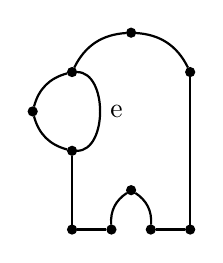
\begin{tikzpicture}[node distance={10mm}, thick, main/.style = {draw,circle,fill,inner sep=1pt}] 
  \node[main] (1) at (0,0) {}; 
  \node[main] (3) at (-0.5,0.5) {}; 
  \node[main] (4) at (0, 1) {}; 
  \node[main] (5) at (0, -1) {}; 
  \node[main] (6) at (1.5, -1) {}; 
  \node[main] (7) at (0.75, 1.5) {}; 
  \node[main] (8) at (1.5, 1) {}; 
  \node[main] (9) at (0.5, -1) {}; 
  \node[main] (10) at (1, -1) {}; 
  \node[main] (11) at (0.75, -0.5) {}; 
  \draw (1) to [bend left] (3);
  \draw (1) to [bend right=90]
node[midway, right] {e} (4) ;
  \draw (3) to [bend left] (4);
  \draw (4) to [bend left] (7);
  \draw (7) to [bend left] (8);
  \draw (8) to (6);
  \draw (5) to (9);
  \draw (6) to (10);
  \draw (9) to [bend left] (11);
  \draw (10) to [bend right] (11);
  \draw (5) to (1);
\end{tikzpicture} 
\end{subfigure}
\begin{subfigure}[h]{0.245\textwidth}
  \caption{$C _1$}
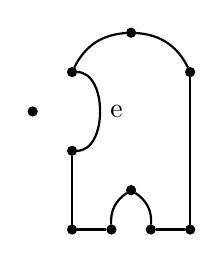
\begin{tikzpicture}[node distance={10mm}, thick, main/.style = {draw,circle,fill,inner sep=1pt}] 
  \node[main] (1) at (0,0) {}; 
  \node[main] (3) at (-0.5,0.5) {}; 
  \node[main] (4) at (0, 1) {}; 
  \node[main] (5) at (0, -1) {}; 
  \node[main] (6) at (1.5, -1) {}; 
  \node[main] (7) at (0.75, 1.5) {}; 
  \node[main] (8) at (1.5, 1) {}; 
  \node[main] (9) at (0.5, -1) {}; 
  \node[main] (10) at (1, -1) {}; 
  \node[main] (11) at (0.75, -0.5) {}; 
  \draw (1) to [bend right=90]
node[midway, right] {e} (4) ;
  \draw (4) to [bend left] (7);
  \draw (7) to [bend left] (8);
  \draw (8) to (6);
  \draw (5) to (9);
  \draw (6) to (10);
  \draw (9) to [bend left] (11);
  \draw (10) to [bend right] (11);
  \draw (5) to (1);
\end{tikzpicture} 
\end{subfigure}
\begin{subfigure}[h]{0.245\textwidth}
  \caption{$C _2$}
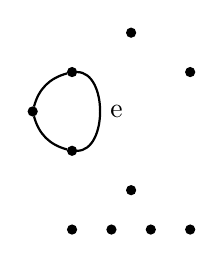
\begin{tikzpicture}[node distance={10mm}, thick, main/.style = {draw,circle,fill,inner sep=1pt}] 
  \node[main] (1) at (0,0) {}; 
  \node[main] (3) at (-0.5,0.5) {}; 
  \node[main] (4) at (0, 1) {}; 
  \node[main] (5) at (0, -1) {}; 
  \node[main] (6) at (1.5, -1) {}; 
  \node[main] (7) at (0.75, 1.5) {}; 
  \node[main] (8) at (1.5, 1) {}; 
  \node[main] (9) at (0.5, -1) {}; 
  \node[main] (10) at (1, -1) {}; 
  \node[main] (11) at (0.75, -0.5) {}; 
  \draw (1) to [bend left] (3);
  \draw (1) to [bend right=90]
node[midway, right] {e} (4) ;
  \draw (3) to [bend left] (4);
\end{tikzpicture} 
\end{subfigure}
\begin{subfigure}[h]{0.245\textwidth}
  \caption{$C _3$} 
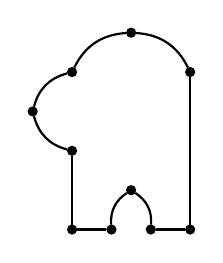
\begin{tikzpicture}[node distance={10mm}, thick, main/.style = {draw,circle,fill,inner sep=1pt}] 
  \node[main] (1) at (0,0) {}; 
  \node[main] (3) at (-0.5,0.5) {}; 
  \node[main] (4) at (0, 1) {}; 
  \node[main] (5) at (0, -1) {}; 
  \node[main] (6) at (1.5, -1) {}; 
  \node[main] (7) at (0.75, 1.5) {}; 
  \node[main] (8) at (1.5, 1) {}; 
  \node[main] (9) at (0.5, -1) {}; 
  \node[main] (10) at (1, -1) {}; 
  \node[main] (11) at (0.75, -0.5) {}; 
  \draw (1) to [bend left] (3);
  \draw (3) to [bend left] (4);
  \draw (4) to [bend left] (7);
  \draw (7) to [bend left] (8);
  \draw (8) to (6);
  \draw (5) to (9);
  \draw (6) to (10);
  \draw (9) to [bend left] (11);
  \draw (10) to [bend right] (11);
  \draw (5) to (1);
\end{tikzpicture} 
\end{subfigure}
                  \end{figure}

% We can say that a set $X \subseteq E$ is independent if and only if, it does not contain any circuit.
% The concept of circuits points towards something similar to a complement of the independent sets, but not completely. It is only the minimal dependent, and not all dependet subsets. We now have the following theorem.

\begin{lemma}\label{lem:circuits-have-properties}
  All circuits in a matroid satisfy (C1), (C2) and (C3).
\end{lemma}

\begin{proof} We will prove each property individually:
  
\begin{enumerate}
    \item[(C1)] $\emptyset \in \mathcal I$, therefore $\emptyset$ is not dependent (which means it cannot be a circuit)
    \item[(C2)] Assume that for $C_1$ and $C_2$ minimally dependent with $C_1\subseteq C_2$, it holds that $C_1\neq C_2$. In other words, $C_1$ is propperly contained in $C_2$. This contradicts the fact that $C_2$ is minimally dependent.
    %A counterexample to this clause would violate $C _2$ being minimal.
    \item[(C3)] Assume a counterexample exists. Because $C _1 \cup C _2 - e$ does not contain a circuit, it must be an element of $\mathcal I$. 

        Aiming for contradiction, suppose that $C _2 - C _1$ is empty. That would imply $C _2 \subseteq C _1$, but $C _1 \neq C _2 $ by (C3), which means that $C _1 $ is a proper subset of $C _2$. As both $C _1 $ and $C _2 $ are members of $\mathcal C$, this violates (C2), and is a contradiction. We can then assume some $f \in C _2 - C _1 $ exists.

        As $C _2$ is minimally dependent, we know that $C _2 - f$ is independent. Let $I$ be a maximal independent subset of $C _2 \cup C _1$ which is a superset of $C _2 - f$. Clearly, $f \not\in I$ (otherwise $C _2 \subseteq I \in \mathcal I$). Furthermore, as $C _1 $ is a circuit, we know that $C _1 \not \subseteq I \in \mathcal I$ (otherwise $C _1$ would be independent). This means some $g \in C _1$ exists such that $g \not\in I$. As $f \in C _2  -  C _2$, we know that $f \neq g$.

        As $I \subseteq C _1 \cup C _2$ and $f, g \in C _1 \cup C _2$ but $f, g \not\in I$, we can infer that 
        \begin{align*}
        |I| \leq |C _1 \cup C _2 - f - g| = |C _1 \cup C _2| - 2.
        \end{align*}

        We also notice that $|C _1 \cup C _2 - e| = |C _1 \cup C _2 | - 1$. We can now conclude by transitivity with $|C _1 \cup C _2 | - 2 < |C _1 \cup C _2 | - 1$ that $|I| < |C _1 \cup C _2 - e|$. We recall that both $I$ and $C _1 \cup C _2 - e$ are members of $\mathcal I$. We can apply (I3) to generate a superset of $I$ which contradicts it's maximality.
\end{enumerate}
\end{proof}

\begin{theorem}\label{thm:matroid-circuit-definition}
Let $E$ be a set and $\mathcal C$ be a collection of subsets of $E$ which satisfies the conditions (C1), (C2) and (C3) outlined above. Let  $\mathcal I$  be the collection of subsets of $E$ that contain no member of $\mathcal C$, that is

\begin{center}
    $ \mathcal{I} = \{I \in 2^E |\; \text{for all } \; C \in \mathcal{C}\; \text{we have} \; C \not\subseteq I\}$
\end{center}
    The pair $(E,\mathcal I)$ is a matroid having $\mathcal C$ as its collection of circuits.
\end{theorem}

\begin{proof} We start by showing that $\mathcal I $ satisfies the necessary conditions for $(E, \mathcal I )$ to be a matroid:
    \begin{enumerate} 
        \item[(I1)] The only subset of $\emptyset $ is $ \emptyset $, but $ \emptyset \not\in \mathcal C $, as $ \emptyset $ satisfies $\mathcal{I}$, $\emptyset \in \mathcal I$.
        \item[(I2)] Assume we have $X \subseteq Y \in \mathcal I$. Aiming for contradiction, assume that $X \not\in I$, i.e.\ there exists some $C \in \mathcal C $ such that $C \subseteq X$. We recall that $\subseteq $ is transitive, thus $C \subseteq Y$ and $Y \not\in I$, hence a contradiction.
        \item[(I3)] Given $X, Y \in \mathcal I $ with $|X| < |Y|$ we must show there exists some $e \in Y - X$ such that $X \cup e \in \mathcal I$. Assume that a counterexample exists. That is, some pair $X, Y \in \mathcal I$ must exist such that for all $e \in Y - X$ we have $X \cup e \not\in \mathcal I$. Assume such a counterexample exists. Pick such a counterexample which maximizes $|X \cap Y|$. Assume $X - Y$ is nonempty (otherwise $X \subseteq Y$ and by (I2) we can pick any $ y\in Y - X$ such that $X \cup y \in \mathcal I$, because $X\cup y\subseteq Y$). Pick some $x \in X - Y$. We will proceed by cases:
          \begin{enumerate}
            \item If $Y \cup x$ is independent, we claim that $(X, Y \cup x)$ is a counterexample as well. This is trivially shown by noticing how $(Y \cup x) - X = Y - X$, so any choice of $e \in (Y \cup x) - X$ is also in $Y-X$, which then implies that $X\cup e\notin \mathcal{I}$.
            %such that $X \cup e$ is independent would invalidate $(X, Y)$ being a counterexample. 
            We note that 
              \begin{align*}
              |X \cap (Y \cup x)| = |(X \cap Y) \cup (X \cap x)| = |(X \cap Y) \cup x|,
              \end{align*}
              but $x \not\in X \cap Y$, so $|(X \cap Y) \cup x| = |X \cap Y| + |\{x\}| = |X \cap Y| + 1$. As $|X \cap Y| + 1 > |X \cap Y|$, we can conclude $(X, Y)$ did not maximize $|X \cap Y|$, hence a contradiction.
            \item Otherwise, $Y \cup x$ is not independent. That is to say, some $C \in \mathcal C$ must exist such that $C \subseteq Y \cup x$. We make the five intermediate claims:
            \begin{enumerate}
              \item There exists some $y \in Y - X$ such that $y \in C$.
                \begin{proof}
                  If there is no such $y$, then $C \subseteq X$. This means that there is a circuit inside $X$, which contradicts the fact that $X \in \mathcal{I}$.
                \end{proof}

                We will make use of this $y$ in the rest of the proof.
              \item It holds that $x \in C$.
                \begin{proof}
                  If this is not the case, we have $C \subseteq Y$, which would imply that $Y \not\in \mathcal I$.
                \end{proof}
              \item The circuit $C$ is the unique circuit with the property $C \subseteq Y \cup x.$
                \begin{proof}
                  Assume another distinct $D \in \mathcal C$ exists such that $D \subseteq Y \cup x$. As $x \in C$ and $x \in D$ (this follows similarly to the proof of $x \in C$), we can conclude that $x \in C \cap D$. 

                  We can now apply (C3) to generate some circuit $C' \subseteq  C \cup D - x$. We recall that $C, D \subseteq Y \cup x$, therefore $C \cup D \subseteq Y \cup x$. Furthermore, $C \cup D - x \subseteq Y$. By transitivity with $C' \subseteq C \cup D - x$ we now have $C' \subseteq Y$, which implies by definition $Y \not\in \mathcal I$, hence a contradiction.
                \end{proof}


              \item $(Y \cup x) - y$ is independent. 

                \begin{proof}
                If this is not the case, there must exist some $D \in \mathcal C$ with $D \subseteq (Y \cup x) - y$. Since $(Y \cup x) - y \subseteq Y \cup x$, this implies that $D$ is a circuit with $D \subseteq Y \cup x$. By the uniqueness $C$ proved before, we have $D = C$. But this would imply that $y\in C = D$ so $y \in (Y \cup x) - y$ which is a contradiction.  
                \end{proof}

              \item $(X, (Y \cup x) - y)$ is a counterexample for (I3).

                \begin{proof}
                  This trivially follows after noticing that 
                  \begin{align*}
                  ((Y \cup x) - y) - X \subseteq (Y \cup x) - X = Y - X.
                  \end{align*}

                  Any choice $e \in ((Y \cup x) - y) - X$ is then also in $Y-X$, which implies that $X\cup e\notin \mathcal{I}$. This is exactly what it means to be a counterexample for (I3).
                  %such that $X \cup e$ is independent would then invalidate $(X, Y)$ being a counterexample, hence a contradiction.
                \end{proof}
            \end{enumerate}

            We now notice that
            \begin{align*}
              |X \cap ((Y \cup x) - y)| &= |(X \cap (Y \cup x)) - y| 
              \\&=  |((X \cap Y) \cup (X \cap x)) - y|
              \\&=  |((X \cap Y) \cup x) - y|.
            \end{align*}

              We note that $y \notin X$ means that $y \neq x$, and therefore $((X \cap Y) \cup x) - y = (X \cap Y) \cup x$. Furthermore, $x\notin Y$ means that $x\not\in X \cap Y$, and therefore $|(X \cap Y) \cup x| = |X \cap Y| + 1$. We can now conclude that $|X \cap ((Y \cup x) - y)| = |X \cap Y| + 1$. As $|X \cap Y| + 1 > |X \cap Y|$ and $(X, (Y \cup x) - y)$ is a counterexample of (I3), we can conclude that $(X, Y)$ did not maximize $|X \cap Y|$, hence a contradiction.
    \end{enumerate}
\end{enumerate}


We now show that $C$ is a circuit for the newly defined matroid if and only if it is a member of $\mathcal C$. 
\begin{enumerate}
  \item[$\implies$]
    If $C$ is a circuit for $(E, \mathcal I)$, then $C \not\in \mathcal I$, which means that $C$ contains some $D \in \mathcal C$. As $C$ is minimally dependent, all its proper subsets are independent, but members of $\mathcal C$ cannot be independent (as seen in the definition of $\mathcal I$), which implies that $C = D$, hence $C \in \mathcal C$.
  \item[$\impliedby$]
    Let $C \in \mathcal{C}$. Since $C\subseteq C$, $C\notin \mathcal{I}$ is implied by how we defined $\mathcal{I}$. The fact that $C$ is now dependent means that there is a set $D$ contained in $C$ that is a circuit of the matroid. We have already shown that a circuit of the matroid is an element of $\mathcal{C}$, which implies that $D\in\mathcal{C}$. Now we can apply (C2) on $D$ and $C$ to see that $C=D$. Thus, $C$ is a circuit of the matroid.
    %Let $C \in \mathcal C$. Assume $C$ is not a circuit for $(E, \mathcal I)$. Clearly, $C \not\in \mathcal I$ is implied by the definition of $\mathcal I$ seen above. This implies that $C$ is dependent but not a circuit, which means $C$ is not miminal. 

  %A proper subset $D  \subsetneq C$ must then exist such that $D$ is a circuit. We have already shown in the $\implies$ direction how this implies $D \in \mathcal{C}$. We have now constructed a contradiction to (C2), hence our assumption that $C \in \mathcal C$ is false.

\end{enumerate}



  We can now conclude that $(E, \mathcal I)$ is indeed a matroid with $\mathcal C$ as it's set of circuits.
\end{proof}

\begin{exmp}
    

We will consider the uniform matroid $U_{2,4}$ and show that it is $\mathbb{F}_3$-representable, while it is not $\mathbb{F}_2$-representable. First, we note that $U_{2,4}= (\{1,2,3,4\}, \mathcal{I})$ where the bases are all of the two element subsets of $\{1,2,3,4\}$. So the matroid looks like: 



\begin{figure}[h]\label{u24}

\begin{center}

\begin{tikzpicture}

\matrix (a) [matrix of math nodes, column sep=0.6cm, row sep=0.6cm,]{
 & & &\textcolor{cyan}{
1234} & & & &\\
 \textcolor{blue}{
123}& &\textcolor{blue}{
124} & &\textcolor{blue}{
134} &  & \textcolor{blue}{
234}  \\
\textcolor{red}{12} & \textcolor{red}{13} & \textcolor{red}{14} & & \textcolor{red}{23} & \textcolor{red}{
24} & \textcolor{red}{
34} \\
\textcolor{orange}{1}& &\textcolor{orange}{2} & & \textcolor{orange}{3}& & \textcolor{orange}{4} \\
& & & \textcolor{orange}{\emptyset} &  & & \\
&&&&&& \\};

\foreach \i/\j in {1-4/2-1, 1-4/2-3, 1-4/2-5, 1-4/2-7, 2-1/3-1, 2-1/3-2, 2-1/3-5, 2-3/3-1, 2-3/3-3, 2-3/3-6, 2-5/3-2, 2-5/3-3, 2-5/3-7, 2-7/3-5, 2-7/3-6, 2-7/3-7, 3-1/4-1, 3-1/4-3, 3-2/4-1, 3-2/4-5, 3-3/4-1, 3-3/4-7, 3-5/4-3, 3-5/4-5, 3-6/4-3, 3-6/4-7, 3-7/4-7, 3-7/4-5, 4-1/5-4, 4-3/5-4, 4-5/5-4, 4-7/5-4}
\draw[double, line width = 0.005mm, color = brown] (a-\i) -- (a-\j);

\node[draw] at (0, -2.5){\small \textcolor{orange}{Independent set}, \textcolor{red}{Basis}, \textcolor{cyan}{Dependent set}, \textcolor{blue}{Circuit} };

\end{tikzpicture}
\end{center}
\caption{Representation of $U_{2,4}$}

\end{figure}

Suppose $U_{2,4}$ were $\mathbb{F}_2$-representable. Then there is some $A = \mat_{m \times 4}(\mathbb{F}_2)$, 

$$A = \begin{pmatrix}
    v_1 & v_2 & v_3 & v_4
\end{pmatrix}$$

so that $U_{2,4} \sim M[A]$. We have the following observation.

\begin{lemma}
\label{f2lema}
    Suppose a set of vectors $A = \{w_1, w_2, \cdots, w_r\} \subseteq \mathbb{F}_2^n$ is minimaly linarly dependent, that means that it is linarly dependent but any proper subset of it is linearly independent. Then $w_1 + w_2 + \cdots + w_r = 0$.
\end{lemma}

\begin{proof}
    Because $A$ is linearly dependent, there exists a set of scalars $\{a_1, a_2, \cdots, a_r\}\in \mathbb{F}_2$ not all zero such that
    
    $$\sum_{i=1}^r a_iv_i = 0.$$
    
    If for some $1\leq j \leq r$ we have $a_j = 0$ then we also have 
    
    $$\sum\limits_{\substack{i = 1 \\ i \neq j}} ^r a_iv_i = 0$$

    but not all out of $a_1, \cdots a_{j-1}, a_{j+1}, \cdots a_r$ are 0. This means that ${v_1, \cdots, v_{j-1}, v_{j+1}, \cdots, v_r}$ is linearly dependent, which is not true by assumption. Therefore, for all $1\leq j \leq r$ we have $a_j \neq 0$. But since the field is $\mathbb{F}_2$ this forces $a_j = 1$ for all $j$. Hence, we obtained what we want, namely

     $$\sum_{i=1}^r a_iv_i = 0 =  \sum_{i=1}^r 1 \cdot v_i = 0.$$
    
\end{proof}

If the matroid $U_{2,4} \sim M[A]$ for the above $A$ then we would have all of the three element subsets of vectors to be minimally linearly dependent. This means by lemma(\ref{f2lema}) that $v_1 + v_2 + v_3 = 0$ and $v_1 + v_2 + v_3 = 0$. However, we are in $\mathbb{F}_2$ so 


$$v_1 + v_2 + v_3 = 0 \iff v_1 + v_2 + (v_3 + v_3) = v_3 \iff v_1 + v_2 = v_3 $$

And in the same way $v_1 + v_2 = v_4$. This implies that
$$v_3 + v_4 = (v_1 + v_2 )+ (v_1 + v_2) = 0$$
so the set $\{v_3, v_4\}$ is linearly dependent, which is a contradiction. So $U_{2,4}$ is not $\mathbb{F}_2$-representable. However, $U_{2,4}$ is $\mathbb{F}_3$-representable. For instance the following matrix taken from \cite[20]{oxley1} works, namely

$$A = \begin{pmatrix}
    1 & 0 & 1 & 1 \\
    0 & 1 & 1 & 2
\end{pmatrix}$$.

 We see that no column vector of $A$ is 0, so all single-element subsets are independent. No vector is a scalar multiple of each other, so two element subsets are independent. Finally, no 3-element subsets can be independent, since the dimension of the $\mathbb{F}_3^2$ is 2, so the dimension of any subspace is at most 2.

To conclude the example of $U_{2,4}$, we will show that $U_{2,4}$ has an interesting property that it is not a graphic matroid. In other words, we can show that there is no graph $G$ such that $U_{2,4} \sim M$ where $M$ is the matroid formed by the set of edgs of $G$ with the usual rules. 

We will show $U_{2,4}$ is not graphic by contradiction, that is assume $U_{2,4}$ is graphic and let $G$ be the graph it represents. Then $G$ has four edges and since all two-element subsets of $U_{2,4}$ are independent we see that $G$ has no loops or parallel edges. In particular, all three-element subsets of $U_{2,4}$ are circuits, so in the graph the edges they correspond to form a cycle. But if both sets $\{1,2,3,\}$ and $\{1,2,4\}$ corresonds to edge cycles without parallel edegs it immediatly follows that $3$ and $4$ connect the same vertices, i.e. are parallel edges, which is a contradiction. It follows that $U_{2,4}$ is not graphic.

%In the succeeding sections, we will also consider an example of a matroid, which is not representable over any field.

\end{exmp}

